\section{Graphics Programming in Haskell}

% OpenGL, Gloss etc

\begin{marginfigure}
	
\includegraphics{res/gloss/gloss-tree.png}
	\vspace{1em}
	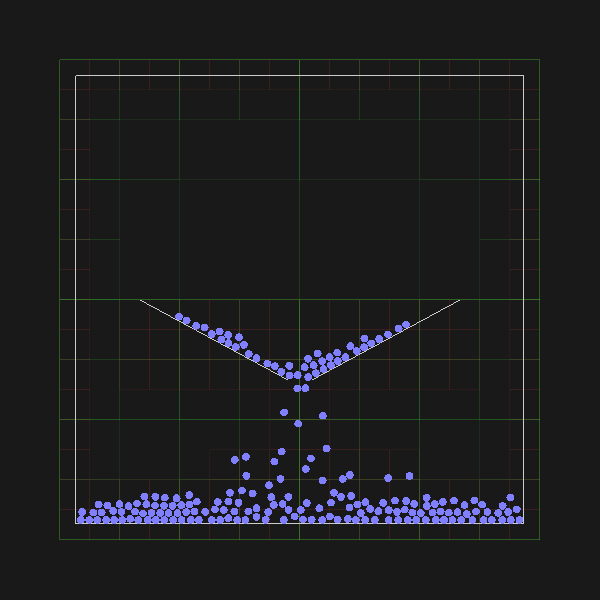
\includegraphics{res/gloss/gloss-styrene.png}
	\caption[Gloss example screens.]{Gloss example screens from \url{gloss.ouroborus.net/}.}
	\label{fig:gloss}
\end{marginfigure}

Any game is clearly going to involve graphics in some capacity or another, but graphics are not something that at first sight seem suited to a functional language. There are, however, various graphical frameworks and bindings available for Haskell.

For the purposes of the Serenity project, the choice basically boiled down to three options. Firstly, there are bindings directly to OpenGL available; which would provide the most flexibility but also likely the most development time. Secondly there are the bindings to the SDL engine, along with all the various tools provided with its framework. Many of the existing games written in Haskell use SDL. Lastly there is the use of the simple but effective layer over GLUT and OpenGL provided by the Gloss library.

This was not an easy decision, and some time went into making it. The direction taken in the Serenity project was to use the Gloss library, mostly because of its simple interface and ease of use, given the limited time and large scope of the rest of the project. The advantages of Gloss can be appreciated by considering the two screens in Figure \ref{fig:gloss}. Both of these examples involve relatively simple code, which is almost entirely pure.

The decision to use Gloss has largely been held up, but there has been some problems due to features it lacks, the most notable being clipping. In the future it would probably be beneficial to replace Gloss with an in house framework providing a layer between the pure graphics code and impure bindings to OpenGL.

Some details of the OpenGL and Gloss approaches are given below to illustrate the differences and tradeoffs involved.

\subsection{Using OpenGL Directly}

\marginnote{{\bf NB} --- The OpenGL code in this section is based on the tutorial at \url{www.haskell.org/haskellwiki/OpenGLTutorial1} (retrieved April 2013).}
Writing OpenGL code in Haskell is in many ways similar to writing it in C++ or any similar language. OpenGL calls are simply functions in the IO monad, (i.e. functions of type "IO a"), and there are some special primitive types such as "GLFloat". 

Listing~\ref{list:openglbasic} shows a very simple example of drawing an empty circle and a filled circle, and the output is shown in Figure~\ref{fig:openglbasicout}. Normal Haskell style is used to create a circle: using the "map" function and some trigonometry. These are then converted into OpenGL actions and rendered in the display callback. 

\vspace{-0.5em}
\begin{listing}{list:openglbasic}{Simple OpenGL example, drawing an empty circle and a filled circle (output shown in Figure~\ref{fig:openglbasicout}.}{Simple OpenGL example, drawing an empty circle and a filled circle (output shown in Figure~\ref{fig:openglbasicout}.}{}
\end{listing}\vspace{-1.5em}

\functions(myPoints, pointToVertex, renderMyPoints, display, main, flush, displayPrimitive, displayCallback, getArgsAndInitialize, mapM_, createWindow, mainLoop, clear, renderPrimitive)
\begin{haskell}

>import Graphics.Rendering.OpenGL
>import Graphics.UI.GLUT

>myPoints :: GLfloat -> [(GLfloat,GLfloat,GLfloat)]
>myPoints r = map (\k -> (r*sin(2*pi*k/n),r*cos(2*pi*k/n),0.0)) [1..n] 
>  where n = 100

>pointToVertex :: VertexComponent a => (a, a, a) -> IO ()
>pointToVertex (x,y,z) = vertex $ Vertex3 x y z

>renderMyPoints :: GLfloat -> IO ()
>renderMyPoints r = mapM_ pointToVertex (myPoints r)

>main = do 
>  (progname, _) <- getArgsAndInitialize
>  createWindow "OpenGL Example"
>  displayCallback $= display
>  mainLoop

>display = do 
>  clear [ColorBuffer]
>  renderPrimitive LineLoop (renderMyPoints 1)
>  renderPrimitive TriangleFan (renderMyPoints 0.5)
>  flush

\end{haskell}
\begin{marginfigure}[-25em]
	\hspace{-2em}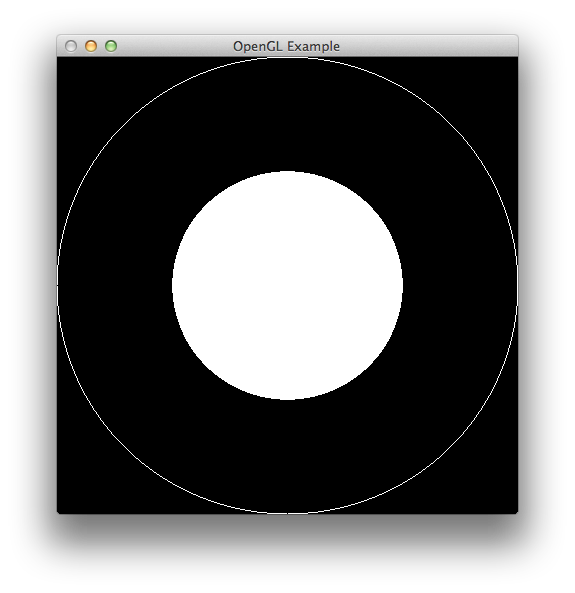
\includegraphics[width=18em]{res/opengl/openglbasic.png}
	\caption[Output of example OpenGL code in Listing~\ref{list:openglbasic}.]{Output of example OpenGL code in Listing~\ref{list:openglbasic}.}
	\label{fig:openglbasicout}
\end{marginfigure}
\vspace{-1em}
\noindent 
The challenge of programming graphics this way is far less an issue of language paradigm than it is of coding style: maintaining a proper separation between the concerns of basic rendering, specific entity models, the game logic, and so on, is the where main engineering effort is required --- and this is no different in Haskell than in other languages. 

As discussed in the previous section, there are various ways that such separation can be achieved, and that primary among these is the concept of an interim type. It is exactly this approach that is taken by the Gloss library, and this is the main reason Gloss was used in Project Serenity, to avoid the additional time it would take to build the infrastructure to work effectively with OpenGL.

\subsection{Using Gloss}

...

\paragraph{Summary of this section} Given the limited time available for the Serenity project, the prebuilt pure interface onto OpenGL provided by the Gloss library was the best option, and this has been born out by the results. A custom made layer that is more appropriate for the needs of a complex game, and more readily adapted to changing requirements, would be beneficial to develop in the future.
